% The six-stage environment step (fig:methodloop). Proposed labels, review 2026-11-24.
% Build:  latexmk -pdf methodloop.tex  -> methodloop.pdf, copy to Images/.
% Fonts match the thesis (lmodern + T1, see styles/myreport.sty).
\documentclass[border=2pt]{standalone}
\usepackage{lmodern}
\usepackage[T1]{fontenc}
\usepackage{amsmath}
\usepackage{tikz}
\usetikzlibrary{positioning,fit,backgrounds,arrows.meta,calc}

% Thesis style: greys only. Shared stages light grey, stage 3 (the only one that differs) a darker grey.
\definecolor{storeF}{HTML}{CFE3F7}
\definecolor{taskF}{HTML}{F6E7C1}
\definecolor{ctrlF}{HTML}{D7F0D8}
\definecolor{estF}{HTML}{F7D6D6}
\definecolor{delF}{HTML}{FFD9B3}
\definecolor{accent}{HTML}{2F6FAE}
\definecolor{ink}{HTML}{43505C}
\definecolor{fb}{HTML}{C0392B}
\definecolor{muted}{HTML}{5A6673}

\definecolor{shareF}{HTML}{F3F5F7}
\definecolor{diffF}{HTML}{DDE1E6}
\tikzset{
  box/.style={draw=ink, line width=0.8pt, rounded corners=3pt, align=center,
              text width=4.1cm, minimum height=1.9cm, inner sep=4pt,
              font=\small},
  insert/.style={draw=ink, line width=0.7pt, fill=white, rounded corners=2pt,
                 font=\scriptsize, inner sep=2pt, minimum height=0.45cm,
                 inner xsep=3pt},
  flow/.style={-{Stealth[length=2.6mm]}, line width=1pt, draw=ink},
  back/.style={-{Stealth[length=2.6mm]}, line width=1pt, draw=ink},
  shared/.style={draw=muted, dashed, rounded corners=6pt, inner sep=6pt},
}

\begin{document}
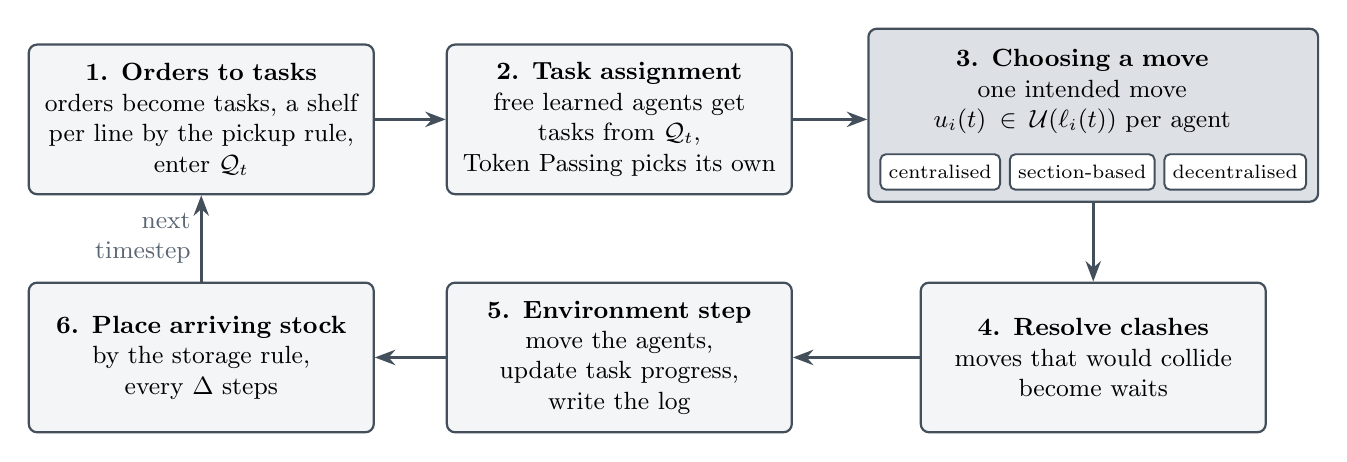
\begin{tikzpicture}
  % top row, left to right
  \node[box, fill=shareF] (O) {\textbf{1. Orders to tasks}\\
    orders become tasks, a shelf\\ per line by the pickup rule,\\ enter $\mathcal{Q}_t$};
  \node[box, fill=shareF, right=0.9cm of O] (A) {\textbf{2. Task assignment}\\
    free learned agents get\\ tasks from $\mathcal{Q}_t$,\\ Token Passing picks its own};
  % stage 3 is a text node plus a row of inserts, framed together
  \node[align=center, font=\small, text width=4.9cm, right=1.1cm of A,
        yshift=0.35cm] (Rt) {\textbf{3. Choosing a move}\\
    one intended move\\ $u_i(t) \in \mathcal{U}(\ell_i(t))$ per agent};
  \node[insert, below=0.12cm of Rt] (i2) {section-based};
  \node[insert, left=0.1cm of i2] (i1) {centralised};
  \node[insert, right=0.1cm of i2] (i3) {decentralised};
  \begin{scope}[on background layer]
    \node[draw=ink, line width=0.8pt, rounded corners=3pt, fill=diffF,
          inner sep=4pt, fit=(Rt)(i1)(i3)] (R) {};
  \end{scope}

  % bottom row, right to left
  \node[box, fill=shareF, below=1.0cm of R] (C) {\textbf{4. Resolve clashes}\\
    moves that would collide\\ become waits};
  \node[box, fill=shareF] (E) at (A |- C) {\textbf{5. Environment step}\\
    move the agents,\\ update task progress,\\ write the log};
  \node[box, fill=shareF] (S) at (O |- C) {\textbf{6. Place arriving stock}\\
    by the storage rule,\\ every $\Delta$ steps};

  \draw[flow] (O) -- (A);
  \draw[flow] (A.east) -- (A.east -| R.west);
  \draw[flow] (R) -- (C);
  \draw[flow] (C) -- (E);
  \draw[flow] (E) -- (S);
  \draw[back] (S) -- node[left, font=\small, text=muted, align=right]
    {next\\ timestep} (O);

\end{tikzpicture}
\end{document}
